\chapter{Setting the Scene for Imperfect Information}
\epigraph{
  Intelligence is a~game of~imperfect information.
  We can guess our opponent's moves, but we can't be sure until the game is over.
}{Khalid Muhammad}
\todo Uvod

\section{Extensive Form for Imperfect-Information}
\label{sec:extensive-form-imperf-info}
\epigraph{
  Education is only a~ladder to~gather fruit from the tree of~knowledge, not the fruit itself.
}{Albert Einstein}
Recall extensive forms (for perfect-information games) from Section~\ref{sec:extensive-form-perf-info}.
An~\emph{extensive form} (for an~imperfect-information game) is the usual extensive form with additional:
\begin{itemize}
  \item \textbf{c}hance player $c$ (e.~g. a~dice, the card dealer, the nature etc.).
    The set of~players is thus $P \cup \braces{c}$ and the probability corresponding to a~strategy profile~$\sigma$ includes the chance:
    \[\pi ^\sigma(h) = \prod _{i \in P \cup {c}} \pi _i ^\sigma (h)\]

  \item function $f_c$ determining the probability distribution over actions~$A(h)$ for every chance node~$h$ (i.e. $p(h) = c$).

  \item partition $\I_i$ of nodes $\braces{h \in H: p(h) = i}$, which is called the \emph{information partition} of player~$i$.
    Its element $I \in \I_i$ is an~\emph{information set} of player~$i$ and $I(h) \in \I_i$ (with $p(h) = i$) denotes the information set containing $h$.

    An information set represents grouping of histories that are indistinguishable from $i$'s point of view.
    In the game of poker, for example, this might be because of  opponents' hidden cards.
\end{itemize}
\noindent
\begin{figure}[H]
  \centering
  \scriptsize
  \def\svgwidth{.7\textwidth}
  \input{../img/strategic-form-tree.pdf_tex}
  \def\captionTitle{An~imperfect-information game tree with information sets}
  \caption[\captionTitle]{\captionTitle{} \\(\cite[p.~67]{AGT07})}
  \label{fig:strategic-form-tree}
\end{figure}

There are further notions related to extensive-form games:
\begin{itemize}
  \item A~\emph{strategy}~$\sigma_i$ of player~$i$ gives a~probability distribution over $A(I)$ at every $I \in \I_i$, and $\pi ^\sigma (I, a)$ is the probability of action $a$ at the information set~$I$.
    Again, $\Sigma_i$ denotes the set of all possible strategies for player~$i$.

  \item The probability $\pi _{-i} ^\sigma (h)$ (or sometimes just briefly $\pi _{-i} (h)$) is the product of~all players' contribution, except for the one of player~$i$:
    \[\pi _{-i} ^\sigma(h) = \prod _{j \in P \setminus \braces{i} \cup \braces{c}} \pi _j ^\sigma (h)\]
    
  \item $\sigma | _{I \goto a}$ denotes the strategy identical to $\sigma$ with the only one exception:
    the action~$a$ is always played at the information set~$I$.

  \item A~\emph{best response} $BR _i (\sigma _{-i})$ (or briefly $BR _i (\sigma)$) of player $i$ for given $\sigma _{-p}$ is such a~strategy $\sigma _i \in \Sigma _i$ that maximizes player's expected utility against others:
    \[ u_i (\sigma) = \max _{\sigma'_i \in \Sigma_i} u_i ((\sigma'_i, \sigma_{-i})) \]

  \item A~\emph{Nash equilibrium} (in the context of extensive-form games) is a~strategy profile $\sigma$ such that no player~$i \in P$ has any incentive to deviate from his strategy.
    In other words, all players are playing best responses against each other:
    \[ \forall i \in P\colon u_i (\sigma) = \max _{\sigma'_i \in \Sigma_i} u_i ((\sigma'_i, \sigma_{-i})) \]

  \item The \emph{counterfactual value} $v _i ^\sigma (I)$ is the expected utility provided that the information set $I$ is reached and all players play according to strategy $\sigma$ with exception of player~$i$, who plays to reach $I$:
    \[ v _i ^\sigma (I) = \sum\limits _{h \in I, \; h' \in Z}
      \frac
      {\pi _{-i} ^\sigma(h) \pi ^\sigma(h,h') u_i(h')}
      {\pi _{-i} ^\sigma (I)} \]

  \item A~\emph{counterfactual best response} $CBR _i (\sigma _{-i})$ (or briefly $CBR _i (\sigma)$) of player~$i$ is a~strategy maximizing the counterfactual value at each information set $I \in \I _i$:
    \[ \pi ^\sigma (I, a) \geq 0
      \; \Longleftrightarrow \;
      v _i ^\sigma (I, a) = \max _{a' \in A(I)} v _i ^\sigma (I, a') \]

    Note that $CBR _i (\sigma)$ is always a best response $BR _i (\sigma)$, but the reverse implication does not need to hold:
    a~best response $\sigma$ can select an~arbitrary action in an~unreachable information set $I$ (the one where $\pi ^\sigma (I) = 0$).
    Such best responses are in general not counterfactual best responses.

  \item For the sake of notation's simplicity, we will define \emph{counterfactual best response value} as the counterfactual value for the strategy, where player $i$ plays according $CBR _i (\sigma _{-i})$ rather than the original $\sigma$.
    Formally, it is
    \[ CBV _i ^\sigma (I) = v _i ^{(\sigma _{-i}, CBR _i (\sigma _{-i} ))} (I) \]

\end{itemize}

There may be various properties for extensive-form games:

\begin{itemize}
  \item being \emph{two-player}
  \item having \emph{perfect recall}: any two states from the same information set $I \in \I _i$ share the same history of past actions and player $i$'s information sets.

    In other words, at any stage of the game no player can forget what happened so far:
    neither actions taken nor the information sets reached.
  \item being \emph{zero-sum}: For any $\sigma \in \Sigma$ we have $\sum _{i \in P} u _i (\sigma) = 0$.
\end{itemize}

\section{Sequence Form}
{
  \setlength{\epigraphwidth}{0.65\textwidth}
  \epigraph{
    Error is ever the sequence of~haste.
  }{Duke of Wellington}
}%
One possible way to~solve extensive-form games is with linear programming (\cite[pp.~73--74]{AGT07}).
However, the number of~pure strategies (over which players are mixing) is generally exponential:
\begin{figure}[H]
  \centering
  \tiny
  \def\svgwidth{.5\textwidth}
  \input{../img/strategic-form-tree.pdf_tex}
  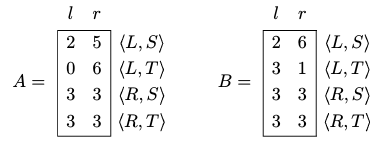
\includegraphics[width=.4\textwidth]{../img/strategic-form.png}
  \def\captionTitle{Left: An~extensive-form game. \\Right: The corresponding strategic-form pay-off matrices.}
  \caption[\captionTitle]{\captionTitle{} \\(\cite[p.~67]{AGT07})}
  \label{fig:strategic-form}
\end{figure}
We need to account for every combination of~actions in~each information set.

Thus, the related linear program (LP) becomes intractable.
A~possible way around this issue is to use the \emph{sequence form} of the game, which reduces the size of LP by having variables only for sequences of~actions and combining only those to obtain a~full game play.

A~\emph{sequence} $s_p(h)$ of~moves of player~$p$ is his history of~actions on the (unique) path from the root to node $h$ while $S_p$ is the set of all possible sequences of player $p$.
The \emph{realization probability} of a~sequence $s_p$ of player~$p$ under a~behavior strategy $\sigma _p$ is $\sigma _p [s] = \prod_{a \in s} \sigma _p(a)$.
It has the meaning of~$p$'s contribution to the product of~probabilities on the sequence $s_p$.
The \emph{realization plan} of some $p$'s mixed strategy $\mu_p$ is a~mapping $x\colon S_p \to \mathbb{R}$ defined by
$x(s) = \sum _{\textrm{pure strategy } \sigma _p} \mu _p (\sigma _p) \cdot \sigma _p [s]$.
We usually write $x$ resp. $y$ for realization plan of player~$1$ resp. player~$2$.
Mixed strategies $\sigma _p, \sigma' _p \in \Sigma _p$ are \emph{realization equivalent} if they reach any game state with equal probabilities, against an~arbitrary strategy of the opponent.
A~well-known result of (Kuhn, 1953)%
\footnote{for further details see \cite{AGT07}}
states that behavior strategies have the same expressive power as mixed strategies:
\begin{thm}[Kuhn's theorem]
For a~player in a~game with perfect recall, any mixed strategy is realization equivalent to some behavior strategy.
\end{thm}
Therefore, we will restrict ourselves to finding equilibria among behavioral strategy profiles, specifically, among possible realization plans.
For any realization plan $x$, any $I \in \mathcal{I}_1$ and any sequence $s\in S_1$, the necessary conditions are
\begin{equation}
\label{seq-cond}
    x(\emptyset) = 1, \quad x(s_1(I)) = \sum _{a \in A(I)} x(s_1(I \cdot a))
\end{equation}
and analogously for any realization plan $y$ of player $2$.
These requirements are natural, since behavior strategies define probability distribution over actions in information sets.

\section{Solving Games with Linear Programming}
{
  \setlength{\epigraphwidth}{0.65\textwidth}
  \epigraph{
    If you optimize everything, you will always be unhappy.
  }{Donald Ervin Knuth}
}%
To describe the conditions (\ref{seq-cond}) as constraints of a~\acrfull{lp}, we think of realization plans as vectors
$(x_s) _{s\in S_1} \equiv x \in \mathbb{R} ^{\lv S_1 \rv}$
and
$(y_s) _{s\in S_2} \equiv y \in \mathbb{R} ^{\lv S_2 \rv}$.
The linear constraints corresponding to (\ref{seq-cond}) are given as
\begin{equation}
\label{seq-constr}
    Ex = e, \ x \ge 0
    \quad \textrm{and} \quad
    Fy = f, \ y \ge 0,
\end{equation}
where the left-hand side is the unit vector $e = (1, 0, \dots, 0) ^\top$ and the constraint matrix
$E \in \mathbb{R} ^{(1 + \lv \mathcal{I}_1 \rv) \times \lv S_1 \rv}$
has columns indexed by all sequences of player~$1$ while rows indexed by the conditions~(\ref{seq-cond}) (similarly also for $F$ and $f$).
Especially, the first row of $Ex = e$ has the form of~$x _{\emptyset} = 1$ and the row corresponding to an~information set~$I \in \mathcal{I}_1$ is
\[
    x _{s_1 (I)} - \sum _{a \in A(I)} x _{s_1(I \cdot a)} = 0.
\]
Analogously for $Fy = f$, that is, $E$ and $F$ are $\{0, -1, 1\}$ matrices.

The sequence form payoff matrix is $A \in \mathbb{R} ^{\lv S_1 \rv \times \lv S_2 \rv}$ for player~$1$ and $-A$ for player~$2$ (as in every zero sum game), which is described for each sequence $s \in S_1$ and each $s' \in S_2$ by
\[
    A _{s,s'} = \sum _{z \in Z,\; s_1(z) = s,\; s_2(z) = s'} u_1(z) \pi_c (z).
\]
Here $\pi_c (z)$ denotes the contribution of~the chance player~$c$ to the overall probability on the path to $z$.
Since this overall probability is the product of~move probabilities on the path to $z$ (including the chance player), the expected utility to player~$1$ is
$
    \sum _{z \in Z} u_1(z) \sigma_1 [s_1(z)] \sigma_2 [s_2(z)] \pi_c (z)
    = x ^\top A y
$
because $\sigma_1 [s_1(z)] = x _{s_1(z)}$ and $\sigma_2 [s_2(z)] = y _{s_2(z)}$.

Now, a~best response $x$ against any fixed plan~$y$ maximizes his expected utility $x ^\top (Ay)$.
In other words, it is a~solution to the LP
\begin{equation}
\label{seq-primal-param}
\begin{split}
    \max\  &x^\top (Ay) \\
    E&x = e \\
    &x \ge 0.
\end{split}
\end{equation}
Its dual linear program has vector $u \in \mathbb{R}^{1 + \lv \mathcal{I}_1 \rv}$ of~unconstrained variables per each equation of~(\ref{seq-primal-param}) and it looks like
\begin{equation}
\label{seq-dual-param}
\begin{split}
    \min\  &u^\top e \\
    E^\top &u \ge Ay.
\end{split}
\end{equation}
As both (\ref{seq-primal-param}) and (\ref{seq-dual-param}) are feasible, they have equal optimal values by the strong duality theorem.
Therefore, whereas player~$1$ wants to maximize $x^\top Ay = u^\top e$, his opponent wants to minimize it (in a~zero sum game) through his free choice of~$y$.
This amounts to the LP
\begin{equation}
\label{seq-dual}
\begin{split}
    \min_{u, y}\  &u^\top e \\
    E^\top u - Ay &\ge 0 \\
    Fy &= f \\
    y &\ge 0
\end{split}
\end{equation}
with the following dual LP
\begin{equation}
\label{seq-primal}
\begin{split}
    \max_{v, x}\  &v^\top f \\
    Ex &= e \\
    F^\top v - A^\top x &\le 0 \\
    x &\ge 0.
\end{split}
\end{equation}
It is important to mention that $E, F, A$ are sparse matrices, whose number of~variables and number of~non-zero values are linear in the size of~game tree.
In conclusion, zero-sum extensive form games can be solved using (dual) linear programming with LPs of~linear sizes.

\section{Solving Games with Learning Algorithms}
{
  \setlength{\epigraphwidth}{0.65\textwidth}
  \epigraph{
    Perfecting oneself is as~much unlearning as~it is learning.
  }{Edsger Wybe Dijkstra}
}%
\todo

\section{Subgames Revisited}

So far, the information sets have grouped only those states where the player was the acting player.
For the purposes of the subgame, it is also necessary to include the states that are indistinguishable from the point of view of other players.
Therefore, we define the \emph{augmented information sets} (\cite{BurchJohansonBowling13}):
\begin{defn}[augmented information set]
  For any player $i \in P$, let $H_i(h)$ be the sequence of player $i$'s information sets reached by player $i$ on the path to $h$, and the actions taken by player~$i$.

  Then \emph{augmented information set} $I_i(h)$ is defined by the following characterization:
  \[ I_i (h) = I_i (h') \; \Longleftrightarrow \; H_i (h) = H_i (h') \]
  for any two states $h, h' \in H$.
\end{defn}
At this point, we may finally define the notion of a~\emph{subgame} (\cite{BurchJohansonBowling13}):
\begin{defn}[subgame]
  \label{defn:subgame}
  An~(imperfect-information) \textbf{subgame} is a~forest of~subtrees, closed under both the descendant relation and membership within augmented information sets for any player.
\end{defn}
Consult Section~\ref{sec:naive-rps-subgame} for an~illustrative example.

\subsection{Previous Works}
